% !TeX spellcheck = en_US
% !TeX encoding = UTF-8
% !TeX root = ../thesis.tex

\chapter{Swarm Reinforcement Learning with Graph Neural Networks}
\label{ch:Architecture}
% pages: 4.26-5.68
First we will introduce the policy architecture used as the base. It is designed to work with PPO and uses the latent node features of the observation for the actor and critic. This base is then expanded with a Graph Neural Network structure that allows multiple hops through a stack of message passing blocks. To support heterogeneous graphs needed for tasks like pursuit the architecture is extended to work on multiple graphs as inputs, but it retains the overarching structure. This makes both GNNs interchangeable. Most of the changes needed for heterogeneous graphs is located in the edge-, node- and global-modules.



\section{PPO - Policy Architecture}
\begin{figure}[htp]
    \centering
    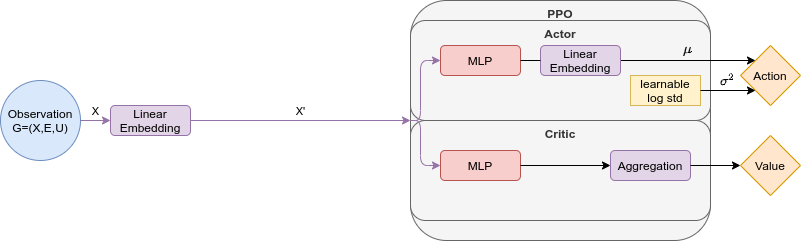
\includegraphics[width=1.0\textwidth]{figures/PPO_no_message_passing.png}
    \hspace{1cm}   
    \caption{Policy architecture used for Swarm Reinforcement Learning with Graph Neural Networks. The node features of the observation graph is the only data used. It is put into a latent dimension and then used by the PPO Network to calculate the action as a distribution and the value.}
    \label{fig:PPO_no_message_passing}
\end{figure}

An overview of the policy architecture can be seen in \Cref{fig:PPO_no_message_passing}.

\begin{itemize}[noitemsep,nolistsep]
    \item Observation as Graph. Graph Generation.
    \begin{itemize}[noitemsep,nolistsep]
        \item Node features is data an agent knows about himself. Edges are observations about neighbors. Notation!
        \item Comparison to Robin. self-observe => Node features,  observe of neighbors => Edge features.
    \end{itemize}
    \item Linear Embedding (Action Dimension => Latent Dimension).
    \begin{itemize}[noitemsep,nolistsep]
        \item Can abstract into a more generalized representation of state observation. That allows for learning relevant relations.
    \end{itemize}
    \item Node features as Input
    \item PPO Architecture Similar to Robin. 
    \item Actor: MLP, Linear Embedding (to Action Space), learnable std (Diag Gaussian).
    \item Critic: MLP, Aggregate (Single Value: min, mean, max), no Embedding (compared to Robin.)
\end{itemize}





\section{Homogeneous Message-passing GNN Architecture}
\begin{figure}[htp]
    \centering
    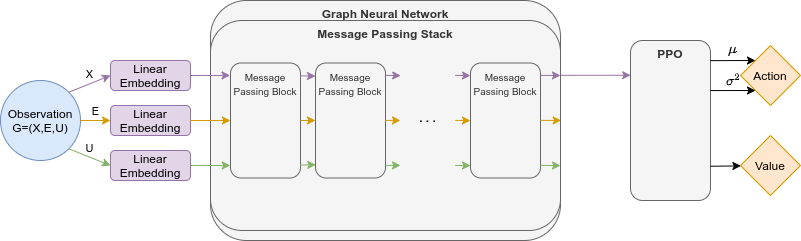
\includegraphics[width=1.0\textwidth]{figures/homogeneous_gnn.png}
    \hspace{1cm}   
    \caption{Here a GNN is added as a step before the policy architecture. The entire observation is put into a latent space and then passed through multiple message passing passes. The outputs of one pass is used as the input of the next pass. This is coordinated through the message passing stack.}
    \label{fig:homogeneous_gnn}
\end{figure}

An overview of the message passing architecture for homogeneous graphs can be seen in \Cref{fig:homogeneous_gnn}.

\begin{itemize}[noitemsep,nolistsep]
    \item Observation Embedding. Nodes, Edges and Globals.
    \begin{itemize}[noitemsep,nolistsep]
        \item No shared weights.
    \end{itemize}
    \item Robin: Basically a Message Passing like structure.
    \begin{itemize}[noitemsep,nolistsep]
        \item For a single observation group:
        \item $f(a_i) = decoder(selfObserve(a_i), \underset{j \in \mathcal{N}_i}{aggr}\ encoder(a_i, observe(a_i, a_j)))$
        \item $f(x_i) = \phi(x_i, \underset{j \in \mathcal{N}_i}{aggr}\ \psi(x_i, x_j))$
    \end{itemize}
    \item GNN composed of Stack. Stack are multiple Message Passing Blocks (a single message passing pass) in sequential order.
    \begin{itemize}[noitemsep,nolistsep]
        \item Easy to create multiple hops.
    \end{itemize}
    \item Block: 3 Modules: Edge-, Node-, Global. How they are wired. Compare that to normal message passing?
    \item Edge-Module:
    \begin{itemize}[noitemsep,nolistsep]
        \item $x_{e'} = f_e(x_v, x_u, x_e, x_g)$
    \end{itemize}
    \item Node-Module:
    \begin{itemize}[noitemsep,nolistsep]
        \item $x_{v'} = f_v(x_v, \oplus_{\{e'=(v,u)||_v\}} x_{e'}, x_g)$
    \end{itemize}
    \item Global-Module:
    \begin{itemize}[noitemsep,nolistsep]
        \item $x_{g'} = f_g(\oplus_V x_{v'}, \oplus_E x_{e'}, x_g)$
    \end{itemize}
    \item Variations/Parameter/Features:
    \item share-base:
    \item aggregation-function used in modules.
    \item use-residual-connections.
\end{itemize}

An overview of the homogeneous message passing block can be seen in \Cref{fig:message_passing_block}.

\begin{figure}[htp]
    \centering
    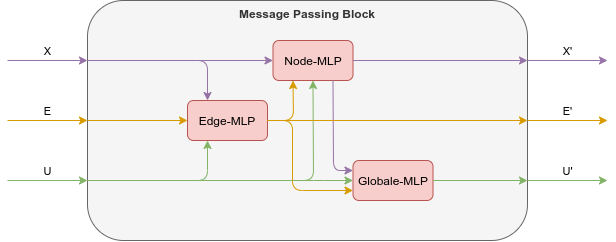
\includegraphics[width=0.75\textwidth]{figures/message_passing_block.png}
    \hspace{1cm}   
    \caption{This is a detailed view of one message passing block. It uses a edge-, node- and global-module to compute a single message passing pass.}
    \label{fig:message_passing_block}
\end{figure}



\section{Heterogeneous Message-passing GNN Architecture}
\begin{figure}[htp]
    \centering
    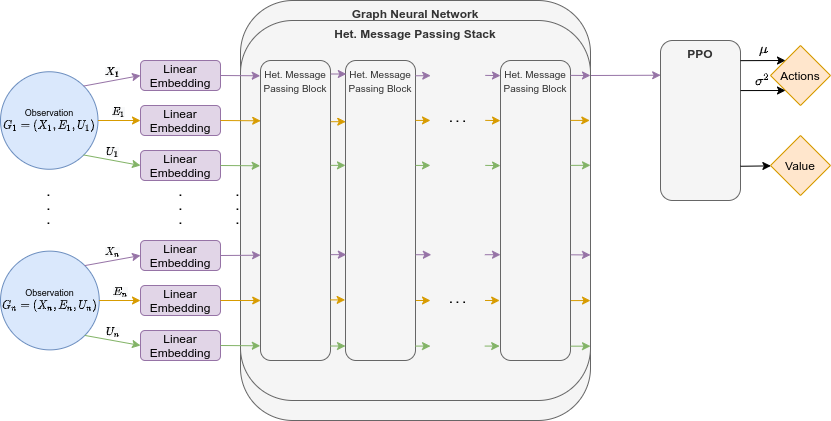
\includegraphics[width=1.0\textwidth]{figures/heterogeneous_gnn.png}
    \hspace{1cm}   
    \caption{An overview of the heterogeneous version of the architecture. The overall structure stays the same, but the input observation is now mulitple graphs. each of the input embeddings per graph is unique. The policy architecture only uses one of the note types as input.}
    \label{fig:heterogeneous_gnn}
\end{figure}

An overview of the message passing architecture for heterogeneous graphs can be seen in \Cref{fig:heterogeneous_gnn}.

\begin{itemize}[noitemsep,nolistsep]
    \item heterogeneous Graphs, MultiGraph. How the data is layed out (math!). Here shown as multiple Graphs.
    \begin{itemize}[noitemsep,nolistsep]
        \item Robin: Needed so that we have support as multiple observation groups. We use heterogeneous graphs.
        \item edge-types, node-types (PyG) => We show it using multiple graphs. (Math!)
    \end{itemize}
    \item Linear Embedder for each type!
    \begin{itemize}[noitemsep,nolistsep]
        \item No shared weights. (Robin: shared weights!) why?
    \end{itemize}
    \item Stacks and Blocks are basically the same, it just now support more inputs.
    \item Edge-Module:
    \begin{itemize}[noitemsep,nolistsep]
        \item $x'_{e_i} = f_{e_i}(x_v, x_u, x_{e_i}, x_g), e_i = (u, v)$
        \item iterate: edge-types -> node-types
    \end{itemize}
    \item Node-Module:
    \begin{itemize}[noitemsep,nolistsep]
        \item $x'_{v'_i} = f_{v_i}(x_{v_i}, [\otimes_j\ \oplus_{\{e_j=(v_i,u)\}} x'_{e_j}], x_g)$
        \item iterate: node-types -> edge-types
    \end{itemize}
    \item Global-Module:
    \begin{itemize}[noitemsep,nolistsep]
        \item $x'_{g} = f_g([\otimes_j\ \oplus_{V_j} x'_{v\in V_j}], [\otimes_k\ \oplus_{E_k} x'_{e\in E_k}], x_g)$
    \end{itemize}
    \item neighbor-aggregation-types concat(aggr()), aggr(aggr())
    \begin{itemize}[noitemsep,nolistsep]
        \item concat(aggr()) (Robin): More expressive, more expensive.
        \item aggr(aggr()) (Robin): less expressive, less expensive. In multi-pursuit: hard to distinguish agents from evaders.
    \end{itemize}
\end{itemize}

An overview of the heterogeneous message passing block can be seen in \Cref{fig:heterogeneous_message_passing_block}.

\begin{figure}[htp]
    \centering
    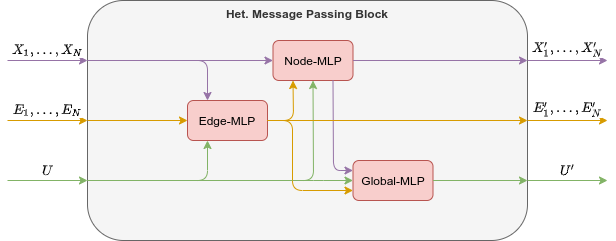
\includegraphics[width=0.85\textwidth]{figures/heterogeneous_message_passing_block.png}
    \hspace{1cm}   
    \caption{Also the structure of the message passing block stays similar. Now the three blocks take all the nodes, edges and global-features of all graphs as input and as output.}
    \label{fig:heterogeneous_message_passing_block}
\end{figure}
